\subsubsection{La tâche de CPT}

\begin{wrapfigure}[7]{l}{2.3cm}
\vspace{-15pt}
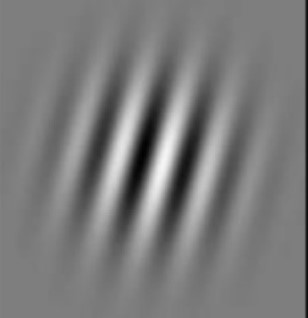
\includegraphics[width=2.3cm]{gabor.jpg}
\captionsetup{labelformat=simpleNumber}
\caption{Gabor}
\end{wrapfigure}

\paragraph{Le dispositif}Le joueur est placé à une distance de 57 cm d'un écran grâce à une mentonnière qui permet de garder une certaine stabilité. Il dispose d'un clavier avec
lequel il se sert uniquement des touches \emph{espace} et \emph{1} et \emph{2} du pavé numérique. Des stimuli sous forme de \emph{\glspl{gabor}} sont présentés au sujet. La cible est un gabor
orienté à 45\degre. Les distracteurs sont des gabors dont l'orientation varie entre 6 et 42\degre par rapport à la cible. Les stimuli apparaissent aléatoirement pendant une période de
80 ms. La cible a une probabilité d'apparition de 12.5\%, soit $1/8$. Pour ne pas donner de rythme à l'apparition des stimuli, un temps d'attente de 200ms à 1 seconde les espace.

\begin{figure}[H]
    \begin{center}
    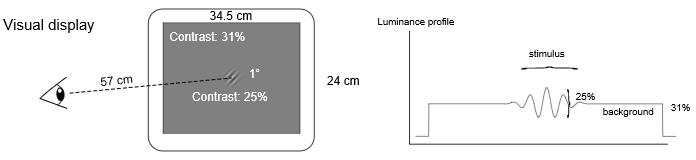
\includegraphics[width=13cm]{cptDispositif.png}
    \end{center}
    \caption{Dispositif de la tâche de CPT et modélisation d'un gabor}
\label{CptDispositif}
\end{figure}

\newpage
\paragraph{}Le sujet a pour objectif de taper sur la barre espace lorsqu'il reconnait la cible. Il dispose d'une seconde après l'apparition de la cible pour répondre. Nous ne cherchons
pas à mesurer les réflexes du sujet mais sa capacité de concentration. S'il trouve la cible, le sujet entend un bip. S'il tape sur un distracteur, il entend un cri. Le sujet a quatre
possibilités de réponses :
\begin{itemize}
\item Il appuie sur une cible. C'est une réponse \emph{correcte} appelée un \textbf{\emph{hit}}.
\item Il n'appuie pas sur un distracteur. C'est une réponse \emph{correcte}.
\item Il appuie sur un distracteur. C'est une réponse \emph{incorrecte} appelée une \textbf{\emph{false alarm}}.
\item Il n'appuie pas sur une cible. C'est une réponse \emph{incorrecte} appelée un \textbf{\emph{miss}}.
\end{itemize}
Le sujet réalise plusieurs séries dans lesquelles il doit trouver la cible 80 fois. La durée complète de l'entrainement dépend des capacités du sujet. Elle oscille généralement entre
1 et 2h pour pouvoir observer des variations durant l'entrainement et des améliorations au fur et à mesure des sessions. Les séries sont entrecoupées d'un test de discrimination.

\begin{figure}[H]
    \begin{center}
    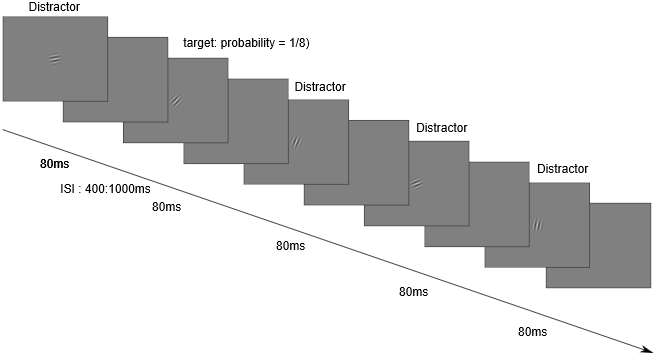
\includegraphics[width=13cm]{cptTask.png}
    \end{center}
    \caption{Exemple d'une partie de série de la tâche de CPT}
\label{CptTask}
\end{figure}

\paragraph{Le test de discrimination}Tout le monde n'a pas la même sensibilité visuelle. Il est donc nécessaire de vérifier la perception du sujet afin de calibrer ses résultats en
fonction. Le dispositif est le même que pour la tâche de CPT. La cible et les distracteurs sont les mêmes. On demande au sujet de fixer un point central et on affiche des couples
cible/distracteur présentées aléatoirement. Un premier stimulus est affiché pendant 80ms, suivi d'un masque pendant 50ms. Ce masque sert à interrompre les post traitements du
stimulus. Puis un écran vierge est présenté pendant 1 secondes. On affiche ensuite le deuxième stimulus du couple de la même manière que le premier. Le sujet doit alors dire si la
cible a été présenté en premier ou en deuxième avec les touches \emph{1} et \emph{2} du pavé numérique. Il a 1.5 secondes pour répondre. Comme pour la tâche de CPT, s'il a juste, il
entend un bip, sinon un cri. Les couples cibles/distracteurs peuvent apparaitre soit au milieu de l'écran en vision centrale, soit légèrement décalé a droite ou a gauche, à la vision
périphérique du sujet. Le test de discrimination dure environ 6 minutes, puis une nouvelle série de la tâche de CPT est lancée.

\begin{figure}[H]
    \begin{center}
    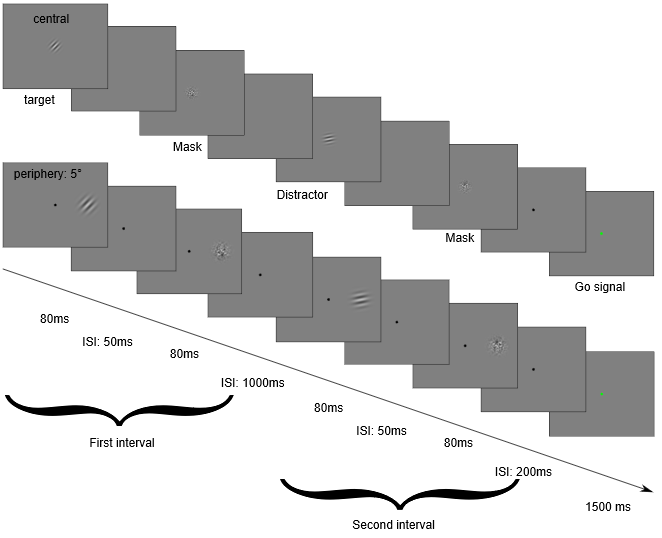
\includegraphics[width=13cm]{cptDiscriminationTask.png}
    \end{center}
    \caption{Exemple d'une partie de test de discrimination}
\label{CptDiscriminationTask}
\end{figure}

\paragraph{Traitement des données}Certaines données sont mémorisées pour être analysées par la suite par les chercheurs. Cela permet de suivre l'évolution de chaque sujet. Mais nous
en parlerons plus en détails dans la partie \ref{Donnees}.
